\section{模型与求解方法}
\label{sec:cone-methods}

同一个问题可以有多种写法。于是要问：写法不同时，变量规模、存储和运算量分别差多少，应该按什么选择？

\paragraph{同一个问题的三种写法}
预算问题已经写过三遍：原变量的二次规划、式~\eqref{eq:cone-qp-socp}的二阶锥形式，以及用式~\eqref{eq:cone-schur-quadratic}得到的线性矩阵不等式。三者等价，解都是$(3/2,1/2)$，规模却不同。表~\ref{tab:cone-three-forms}列出例子（$n=2$，$k=3$）和一般情形。

\begin{BookInlineTable}
  \centering
  \begin{tabular}{llll}
    \toprule
    & 二次规划 & 二阶锥形式 & 线性矩阵不等式\\
    \midrule
    变量 & $2$（一般$n$） & $3$（$n+1$） & $3$（$n+1$）\\
    非线性结构 & $\bm{Q}$，$2\times2$ & $5$维锥（$k+2$） & $4\times4$（$k+1$阶）\\
    矩阵独立元素 & $3$ & 无 & $10$\\
    恢复原变量 & 直接 & 丢弃$t$ & 丢弃$t$\\
    \bottomrule
  \end{tabular}
  \caption{预算问题的三种等价写法。括号内是一般规模：$n$个变量，$\bm{F}\in\mathbb{R}^{k\times n}$。线性约束三者相同，未列出。}
  \label{tab:cone-three-forms}
\end{BookInlineTable}

\paragraph{模型的包含关系}
图~\ref{fig:cone-hierarchy}把前面的改写连成一条链。线性规划是$\bm{Q}=\bm{0}$的二次规划；凸二次规划由式~\eqref{eq:cone-qp-socp}写成二阶锥规划；二阶锥规划由式~\eqref{eq:cone-soc-as-lmi}写成半正定规划。

\begin{BookInlineFigure}
  \centering
  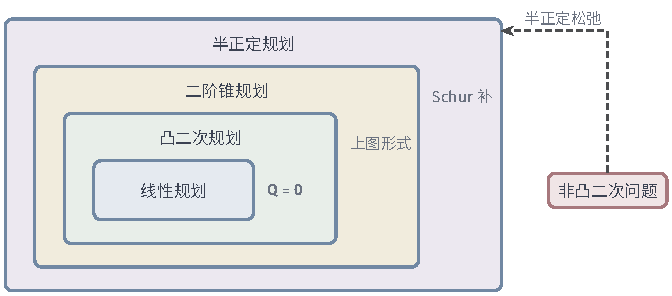
\includegraphics[width=112mm]{figures/05-optimization/06-constrained-optimization/tikz/cone-hierarchy/figure.pdf}
  \caption{模型的包含关系。边框旁标注内层写成外层所用的改写。非凸二次问题不在这条链上，它只能经半正定松弛（虚线）得到下界。}
  \label{fig:cone-hierarchy}
\end{BookInlineFigure}

这条链说的是表达能力，不是推荐的求解路线。外层的模型能表达内层的问题，但内层的结构在外层看不见了。一个$k+2$维的二阶锥写成线性矩阵不等式后，要用$(k+1)\times(k+1)$的矩阵，存储从$O(k)$变成$O(k^2)$。

内点法每步解一个线性方程，按稠密数据粗略估计：$n$个变量的二次规划，每步约$O(n^3)$次运算；变量为$n$、矩阵阶为$k$的线性矩阵不等式，组装牛顿方程的系数矩阵就要$O(nk^3+n^2k^2)$次，分解再要$O(n^3)$次\scite{math-boyd2004convex}。所以能用内层模型时就不要往外走。

\paragraph{松弛的规模}
半正定松弛的规模增长更快。问题~\eqref{eq:cone-sign-relax}把$n$个变量换成$n\times n$的矩阵。$n=1000$时，矩阵存储$10^6$个数，独立的非对角元有$n(n-1)/2=499500$个，一次特征分解约$10^9$次运算。此外还要重复取整和验证。松弛的结果换来的是一个下界，这个下界是否值得这样的代价，要看问题规模和对全局证据的需要。

\paragraph{各类方法的去向}
后面几章给出具体的算法，这里只说明各自处理什么情形。第~\ref{chap:sequential-quadratic-programming}章把二次规划当作子问题反复求解。第~\ref{chap:nonlinear-interior-point}章把第~\ref{chap:lp-interior-point}章的内点法推广到一般光滑约束和锥约束。

若可行集的投影便宜，或约束可以拆成几块分别处理，第~\ref{chap:feasible-iterations}章和第~\ref{chap:penalty-multiplier-methods}章的方法每步代价低得多，适合只需中等精度的大规模问题。

投影到半正定锥就是一个例子：作谱分解，把负特征值截成零。例如$\begin{bmatrix}1&2\\2&1\end{bmatrix}$的特征值是$3$和$-1$，特征向量是$(1,1)/\sqrt2$和$(1,-1)/\sqrt2$。截断负特征值后得到
\[
 3\cdot\frac12\begin{bmatrix}1&1\\1&1\end{bmatrix}=\frac32\begin{bmatrix}1&1\\1&1\end{bmatrix}.
\]
一次投影需要一次完整的特征分解，代价约$O(n^3)$，这决定了这类方法能处理的矩阵阶数。

\paragraph{选择的依据}
选择模型时可以按下面的顺序问。

\begin{enumerate}
 \item 问题是否凸？不凸的话，改写不会改变这一点，只能走局部方法或松弛。
 \item 能否停留在最内层的模型？线性约束的凸二次问题就用二次规划，不要因为通用求解器方便而升级。
 \item 数据有什么结构？稀疏、低秩或只能做矩阵向量积，决定是否可以分解，也决定内点法和一阶方法哪个更合算。
 \item 需要什么样的结论？只要一个好的解，局部方法足够；需要全局证据，就要付出松弛和对偶验证的代价。
\end{enumerate}

无论走哪条路，得到结果后都要分别核对，如图~\ref{fig:cone-workflow}所示。等价改写的解丢弃辅助变量后可以直接用，松弛的解则要先恢复再验证。

\begin{BookInlineFigure}
  \centering
  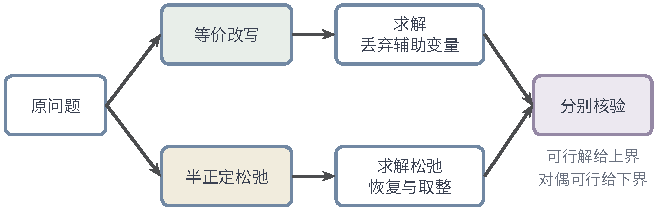
\includegraphics[width=110mm]{figures/05-optimization/06-constrained-optimization/tikz/cone-workflow/figure.pdf}
  \caption{从原问题到可靠结论的两条路径。等价改写（绿）保持最优解，求解后丢弃辅助变量。半正定松弛（黄）扩大可行集，求解后要恢复原变量。两条路径最后都要分别核验：可行解给出上界，对偶可行解给出下界。}
  \label{fig:cone-workflow}
\end{BookInlineFigure}
